\documentclass[12pt]{article}

% Packages
\usepackage[margin=1.2in]{geometry}
\usepackage{graphicx} 
\usepackage{enumerate}
\usepackage{listings}
\usepackage{titling}
\usepackage{multirow}
\usepackage{tabularx}
\usepackage{longtable}
\usepackage{booktabs}
\usepackage{hyperref}
\usepackage{makecell}
\usepackage{caption}
\usepackage{array}
\usepackage{float}
\usepackage{placeins}
\usepackage{float}
\lstset{basicstyle=\small\ttfamily,xleftmargin=18pt,breaklines=true}
\captionsetup[table]{skip=2pt}

% Comments --------------------------------------------------------------------
\usepackage{xcolor}
\newif\ifcomments\commentstrue
\ifcomments \newcommand{\authornote}[3]{\textcolor{#1}{[#3 ---#2]}}
\newcommand{\todo}[1]{\textcolor{red}{[TODO: #1]}} \else
\newcommand{\authornote}[3]{} \newcommand{\todo}[1]{} \fi
\newcommand{\wss}[1]{\authornote{magenta}{SS}{#1}}
\newcommand{\ds}[1]{\authornote{blue}{DS}{#1}}
\newcommand{\mmp}[1]{\authornote{green}{MP}{#1}}
\newcounter{TestCounter}
\setcounter{TestCounter}{0}
% End Comments ---------------------------------------------------------------

\setlength\parindent{0pt} % Cleaner look
\usepackage{xcolor}
\hypersetup{
    colorlinks,
    linkcolor={red!50!black},
    citecolor={blue!50!black},
    urlcolor={blue!80!black}
}

% Title Page -----------------------------------------------------------------
\title{
\LARGE GEANT4 GPU Port:
\\\vspace{10mm}
\large \textbf{Test Report}
\vspace{40mm}
}
\author{
Stuart Douglas -- dougls2
\\Matthew Pagnan -- pagnanmm
\\Rob Gorrie -- gorrierw
\\Victor Reginato -- reginavp
\vspace{10mm}
}
\date{\vfill \textbf{Version 0}\\ \today}
% End Title Page -------------------------------------------------------------

% ============================== BEGIN DOCUMENT ============================= %
\begin{document}
\pagenumbering{gobble} % start numbering after TOC

% ============================== Title Page ============================= %
\maketitle
\newpage

% ================================= TOC ================================= %
\newgeometry{bottom=1.1in, top=1.1in}
\tableofcontents
\newpage
\pagenumbering{arabic}
\restoregeometry

% =============================== Section =============================== %
\section*{Revision History}
All major edits to this document will be recorded in the table below.

\begin{table}[h]
\centering
\caption{Revision History}\label{Table_Revision}
\begin{tabular}{lll}
\toprule
\bf Description of Changes & \bf Author & \bf Date\\\midrule
Added expected vs actual subsection & Matt & 2016-04-23\\
Initial draft of document & Matt, Rob, Victor, Stuart & 2016-03-18\\
Template of document & Matt  & 2016-03-15\\
\bottomrule
\end{tabular}
\end{table}

% =============================== Section =============================== %
\section*{List of Tables}
Tables for specific unit and system tests have been omitted in order to keep this document readable.
\begin{center}
\begin{tabular}{cl}
\toprule
\bf Table \# & \bf Title\\\midrule
\ref{Table_Revision} 			& Revision History\\
\ref{Table_DefAndAcro} 			& Definitions and Acronyms\\
\ref{gen_var_table}			& General Unit Test Variables\\
\ref{Table_SystemTests} & Summary of System Tests\\
\ref{Table_TestsAndRequirements}	& Tests and Requirements Relationship\\
\ref{Table_TestsAndModules}		& Tests and Modules Relationship\\
\bottomrule
\end{tabular}
\end{center}

\section*{List of Figures}
Described here are a list of figures used in this document.
\begin{center}
\begin{tabular}{cl}
\toprule
\bf Figure \# & \bf Title\\\midrule
\ref{figPerformanceInit} & Performance results for \texttt{Init} function\\
\ref{figPerformanceSampleLin} & Performance results for \texttt{SampleLin} function\\
\ref{figPerformanceTimes} & Performance results for \texttt{Times} function\\
\ref{figPerformanceGetXSec_e} & Performance results for \texttt{GetXSec(e)} function\\
\ref{figPerformanceGetXSec_e_min} & Performance results for \texttt{GetXSec(e,min)} function\\
\ref{figPerformanceGet15Percent} & Performance results for \texttt{Get15PercentBorder} function\\
\ref{figPerformanceGet50Percent} & Performance results for \texttt{Get50PercentBorder} function\\
\bottomrule
\end{tabular}
\end{center}

\section*{Definitions and Acronyms} % Matt
This section contains a table of Definitions and Acronyms used within this document.
\begin{table}[h]
\centering
\caption{Definitions and Acronyms}\label{Table_DefAndAcro}
\begin{tabularx}{\textwidth}{lX}
\toprule
\bf Term & \bf Description\\\midrule
GEANT4 & Open-source software toolkit used to simulate the passage of particles through matter\\
GEANT4-GPU & GEANT4 with some computations running on the GPU\\
GPU & Graphics processing unit, well-suited to parallel computing tasks\\
CPU & Computer processing unit, general computer processor well-suited to serial tasks\\
CUDA & Parallel computing architecture for general purpose programming on GPU, developed by NVIDIA\\
Hadr04 & Example simulation installed by default with Geant4, used for system tests.\\
\Xhline{2\arrayrulewidth}
\end{tabularx}
\end{table}

\ds{Your table is in the wrong place for this heading. You might want to add some text in before the table (referencing it) to avoid an empty, floating heading.}
\mmp{Added text to fix floating table issue}

% =============================== Section =============================== % ------------------------- Rob
\section{Introduction}\label{Introduction}
\subsection{Purpose of the Document}
This document summarizes the testing and test conclusions of the GEANT4-GPU project. This document uses the implementation outlined in the test plan.

\subsection{Scope of the Testing}
The implemented tests are designed to give a general yet rigorous assessment of the components involved in terms of accuracy and performance.\\

The tests are separated into two categories: unit tests and system tests. There are a large number of unit tests which test single functions of the modified G4ParticleVector module, comparing results of the function call with specified inputs between the existing CPU-based implementation and the GPU-based implementation of GEANT4-GPU. The system tests run a complete simulation, and the resulting output values are compared between the CPU and GPU implementations. Performance data is recorded for each performance test.\\

Neither the unit tests nor the system tests are concerned with the correctness of the original, CPU-based GEANT4 program, as these runs are used as the baseline for the correctness of GEANT4-GPU modules.\\

A basic knowledge of programming concepts and command-line tools is assumed, as well as familiarity with GEANT4.

\subsection{Organization}
\ds{Use refs for your section/figure/table numbering. That way they'll be auto-generated.\\}
\mmp{Added refs for section}

In Section \ref{Introduction} we provide an introduction to this report. Section \ref{Unit Testing} describes the test cases which are carried out on each function. Section \ref{System Tests} describes system test cases that were carried out by our team. In section \ref{Traceability} traceability matrices to requirements and modules are documented. Section \ref{Changes after Testing} provides a summary of changes made in response to the testing results.

\subsection{Usability Testing}
GEANT4-GPU is a back end implementation of already existing GEANT4 modules. Therefore users will not be interacting with is directly. Since there is no direct user interaction with GEANT4-GPU, usability tests do not fit the project and are not included.

\subsection{Robustness Testing}
The GEANT4-GPU functions are meant to mimic the already existing GEANT4 functions. Therefore the GEANT4-GPU functions must also mimic the the robustness of the GEANT4 functions. The accuracy section for unit tests has several unit tests designed to test the robustness of the functions, so robustness is included in accuracy results.

% =============================== Section =============================== 
\section{Unit Testing} \label{Unit Testing}
\subsection{Use of Automated Testing}
\subsubsection{Overview}
Our unit testing system is semi-automated. The user runs a program to generate a test results text file, inputting whether or not Geant4 was compiled with CUDA enabled or disabled. Then, they recompile Geant4 in the opposite configuration (i.e. with CUDA enabled if previously disabled, and vice versa) and run the test program again. At this point there will be two test results text files, one for CUDA enabled, and one for CUDA disabled. In addition, two text files containing runtimes of all computationally-intensive functions are produced. After generating the files, a program to analyze the results is run outputting whether each test case passed or failed, and creating an Excel document (.csv) with the running times.

\subsubsection{Generating Test Results}
\texttt{GenerateTestResults} first initializes several G4ParticleHPVector objects from data files included with Geant4 of varying numbers of entries, including the creation of one G4ParticleHPVector with 0 entries. After the vectors have been initialized, the unit-tested methods are tested with a variety of input values. These cover edge cases (i.e. negative index for array, index greater than number of elements etc.) as well as more ``normal'' cases. The result of each function is then written to the results text file. This can be a single value in the case of ``clean'' functions that simply return a value, or it could be the state of the G4ParticleHPVector object, that is the array of points stored by that object. For performance reasons, instead of writing out the entire array of points, a hash value is generated from the array and is outputted. The value of the input variable for each function call is also outputted, so the results for specific inputs can be analyzed.

\subsubsection{Analyzing Test Results}
After the above files are generated, the \texttt{AnalyzeTestResults} utility runs through both documents and for each unit test outputted its status. If it failed, then the result from the CPU and from the GPU are both printed out. After the analysis completes, the total number of tests passed is outputted. In addition, \texttt{AnalyzeTestResults} will read the files containing runtimes for each function and output them in .csv format to simplify performance analysis.

\subsubsection{How to Run Unit Tests}
The following steps are also recorded in a README file in the \texttt{tests} directory. It is assumed that there is a working copy of GEANT4 on the user's system, set up as per the installation instructions of GEANT4-GPU. In particular, the \emph{geant4.10.02-install} directory must be in the same directory as the \emph{geant4.10.02} directory.\\

\textbf{Generating Test Results:}
\begin{enumerate}
\item Build Geant4 with CUDA disabled (see project README for more information).
\item Run \texttt{make clean} to remove any old files.
\item Run \texttt{make} to build the executable files for generating and analyzing the test results.
\item Execute \texttt{./GenerateTestResults 0}, where 0 indicates that GEANT4 was compiled with CUDA disabled.
\item Rebuild Geant4 with CUDA enabled, and repeat steps 2-4.
\end{enumerate}

At this point, there should be 4 text files in the tests directory. These contain the unit test results and runtimes, respectively, for each of the CPU and GPU runs.\\

\textbf{Analyzing Test Results:}
\begin{enumerate}
\item After generating the test results as outlined above, simply run \texttt{./AnalyzeTestResults}. The result of each individual test will be printed to the terminal.
\item A csv file will be created to easily compare runtimes of each function with CUDA enabled and disabled.
\end{enumerate}


\subsubsection{Note About Random Results}
Some of the tests run in \texttt{GenerateTestResults} are based off of random numbers, which differ between the CPU and GPU implementations. To counteract this, each of those tests is run multiple times and the result is averaged. When analyzing results for those functions, they are only marked as failed if the difference in the values of the GPU and CPU results are more than a specified tolerance. There are some functions that depend on random numbers that modify the data array. Since a hash is outputted and will differ no matter how small the difference in the values of the array are, before hashing the values are all rounded to a lower precision (10 decimal places). This rounding to a lower precision is the tolerance.

\subsection{Definition of Variables Used for Unit Testing}
The following are variables that are used for multiple unit tests. Instead of defining them again for each unit test they are defined here only once. Other variables used for specific unit tests will be defined in their respective unit test sections\\
For all unit tests:
\begin{table}[H]
\centering
\caption{General Unit Test Variables}\label{gen_var_table}
\begin{tabular}{lll}
\toprule
	\bf Name & \bf Type & \bf Description\\\midrule
	n 	& G4double 			& number of entries in the G4ParticleHPVector\\
	r1 	& G4double 			& -1.0\\
	r2	& G4double			& 0.0\\
	r3 	& G4double 			& 0.00051234\\
	r4 	& G4double 			& 1.5892317\\
	r5 	& G4double 			& 513.18\\
	vec0 & G4ParticleHPVector 	& 0 entries\\
	vec1 & G4ParticleHPVector	& 80 entries\\
	vec2 & G4ParticleHPVector 	& 1509 entries\\
	vec3 & G4ParticleHPVector 	& 8045 entries\\
	vec4 & G4ParticleHPVector 	& 41854 entries\\
	vec5 & G4ParticleHPVector 	& 98995 entries\\
	vec6 & G4ParticleHPVector 	& 242594 entries\\
\bottomrule		
\end{tabular}
\end{table}

\ds{Where do you define your tolerance?} \mmp{addressed where we define our tolerance in the note about random results}

\subsection{void Init(istream \& aDataFile, G4int total, G4double ux, G4double uy)} 
	Initializes the data in the current vector with \texttt{total} data points from \texttt{aDataFile}. Each data
	point is multiplied by factor \texttt{ux} for the x-value and \texttt{uy} for the y-value.

	\subsubsection{Test Inputs}
		Each vector \emph{vec1}, \emph{vec2} \ldots \emph{vec6} is associated with a data file, which is the input \texttt{aDataFile} to
		the \texttt{Init} function. These data files are bundled with Geant4, and include measured data points for 
		a given isotope of an element. \texttt{vec0} is not initialized with a data file, as it is meant to be an empty vector to test edge cases.
		As such, \texttt{vec0} is not tested with this function.
		\begin{table}[H]
		\centering
		\caption{Unit Tests - \texttt{Init}}\label{Init_unit}
		\begin{tabular}{lllll}
		\toprule
		\multirow{2}{*}{\bf Test \#}  & \multicolumn{2}{c}{\bf Inputs}\\
		& \bf \texttt{aDataFile} & \bf \texttt{G4int} & \bf \texttt{ux} & \bf \texttt{uy}\\\midrule
		\refstepcounter{TestCounter}\arabic{TestCounter}\label{Init_0} & Current data file & n & 1 & 1\\
		\bottomrule
		\end{tabular}
		\end{table}
	\subsubsection{Test Results}
		\begin{table}[H]
		\centering
		\caption{Test Results -- Init}\label{Init_acc}
		\begin{tabular}{cllllll}
		\toprule
		\multirow{2}{*}{\bf Test \#} & \multicolumn{6}{c}{\bf Test Result}\\
		& vec1 & vec2 & vec3 & vec4 & vec5 & vec6\\\midrule
		\ref{Init_0} & Pass & Pass & Pass & Pass & Pass & Pass\\
		\bottomrule
		\end{tabular}
		\end{table}
	\subsubsection{Performance}
    	\begin{figure}[H]
    	\centering
    	\caption{Performance results for \texttt{Init} function}\label{figPerformanceInit}
    	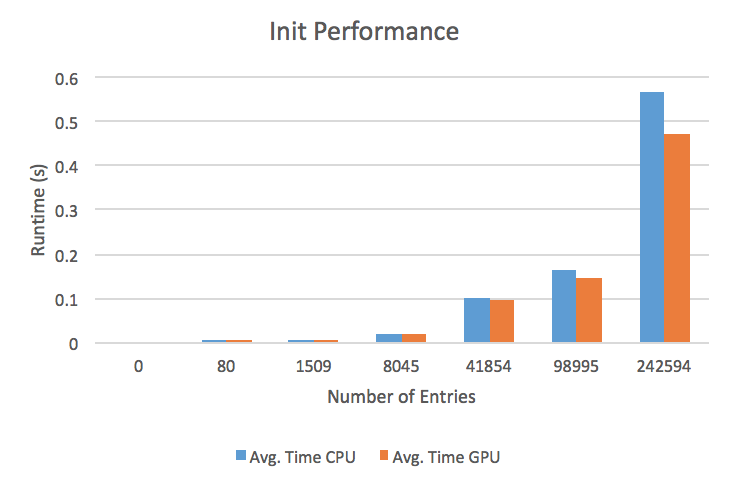
\includegraphics[width=0.7\textwidth]{init_bar.png}
    	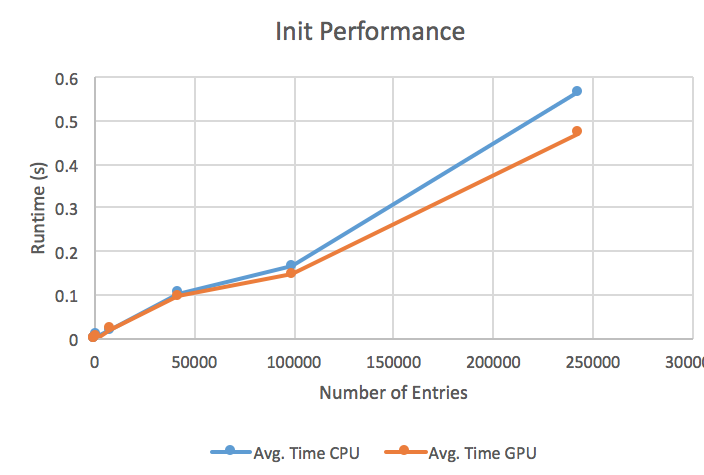
\includegraphics[width=0.7\textwidth]{init_line.png}
   	\end{figure}
	\subsubsection{Expected vs. Actual output}
	We expected to see a performance increase as the size of the vector increased. We also expected the results on the GPU to be the same as on 		the CPU.\\
	The actual output did show a performance increase as teh size of the vector grew, however it was not as large of an increase as we were 	 		expecting. The results on the GPU and CPU were both the same, as expected. 

\subsection{G4ParticleHPVector \& operator = (const G4ParticleHPVector \& right)}
	Create a new, temporary G4ParticleHPVector object and assign the current vector to it. Outputs the data and the integral from the new vector.

	\subsubsection{Test Inputs}
		\begin{table}[H]
		\centering
		\caption{Unit Tests - \texttt{=} (overloaded assignment operator)}\label{OperatorEquals_unit}
		\begin{tabular}{cl}
		\toprule
		\multirow{2}{*}{\bf Test \#}  & \multicolumn{1}{c}{\bf Inputs}\\
		& \bf \texttt{right}\\\midrule
		\refstepcounter{TestCounter}\arabic{TestCounter}\label{OperatorEquals_0} & Current vector\\
		\bottomrule
		\end{tabular}
		\end{table}	
		
	\subsubsection{Results}
		\begin{table}[h]
		\centering
		\caption{Test results - \texttt{=} (overloaded assignment operator)}\label{OperatorEquals_acc}
		\begin{tabular}{clllllll}
		\toprule
		\multirow{2}{*}{\bf Test \#} & \multicolumn{7}{c}{\bf Test Result}\\
		& vec0 & vec1 & vec2 & vec3 & vec4 & vec5 & vec6\\\midrule
		\ref{OperatorEquals_0} & Pass & Pass & Pass & Pass & Pass & Pass & Pass\\
		\bottomrule
		\end{tabular}
		\end{table}

%\ds{The way this is written is very hard to understand. Can you explain it in more depth? 
%Or give a brief rundown of the system state, what the input to each parameter is, etc.?}		% -- commented this out cause it just don't know what Dan meant by this
		
	\subsubsection{Performance}	
		This method is not computationally heavy, so performance data was not included.

	\subsubsection{Expected vs. Actual output}
	 We expected the results on the GPU to be the same as on the CPU.\\
	 The results on the GPU and CPU were both the same, as expected. 
		
\subsection{const G4ParticleHPDataPoint GetPoint(G4int i)}
	
	Returns the G4ParticleHPDataPoint at index \texttt{i} in the current vector. The \texttt{x} 
	and \texttt{y} values of the point are outputted.
	
	\subsubsection{Test Inputs}
		\begin{table}[H]
		\centering
		\caption{Unit Tests - \texttt{GetPoint}}\label{GetPoint_unit}
		\begin{tabular}{lll}
		\toprule
		\multirow{2}{*}{\bf Test \#}  & \multicolumn{1}{c}{\bf Inputs}\\
		& \bf \texttt{i}\\\midrule
		\refstepcounter{TestCounter}\arabic{TestCounter}\label{GetPoint_0} & -1\\
		\refstepcounter{TestCounter}\arabic{TestCounter}\label{GetPoint_1} & 0\\
		\refstepcounter{TestCounter}\arabic{TestCounter}\label{GetPoint_2} & n/2\\
		\refstepcounter{TestCounter}\arabic{TestCounter}\label{GetPoint_3} & n-1\\
		\refstepcounter{TestCounter}\arabic{TestCounter}\label{GetPoint_4} & n\\
		\bottomrule
		\end{tabular}
		\end{table}
	
	\subsubsection{Test Results}
		\begin{table}[H]
		\centering
		\caption{Test Results -- GetPoint}\label{GetPoint_acc}
		\begin{tabular}{clllllll}
		\toprule
		\multirow{2}{*}{\bf Test \#} & \multicolumn{7}{c}{\bf Test Result}\\
		& vec0 & vec1 & vec2 & vec3 & vec4 & vec5 & vec6\\\midrule
		\ref{GetPoint_0} & Pass & Pass & Pass & Pass & Pass & Pass & Pass\\
		\ref{GetPoint_1} & Pass & Pass & Pass & Pass & Pass & Pass & Pass\\
		\ref{GetPoint_2} & Pass & Pass & Pass & Pass & Pass & Pass & Pass\\
		\ref{GetPoint_3} & Pass & Pass & Pass & Pass & Pass & Pass & Pass\\
		\ref{GetPoint_4} & Pass & Pass & Pass & Pass & Pass & Pass & Pass\\
		\bottomrule
		\end{tabular}
		\end{table}
	\subsubsection{Performance}
		This method is not computationally heavy, so performance data was not included.

	\subsubsection{Expected vs. Actual output}
		 We expected the results on the GPU to be the same as on the CPU.\\
	 	The results on the GPU and CPU were both the same, as expected.
		
\subsection{G4double GetX(G4int i)}
	
	Returns the energy at index \texttt{i} in the current vector. The \texttt{x} 
	value of the point are outputted.
	
	\subsubsection{Test Inputs}
		\begin{table}[H]
		\centering
		\caption{Unit Tests - \texttt{GetX}}\label{GetX_unit}
		\begin{tabular}{lll}
		\toprule
		\multirow{2}{*}{\bf Test \#}  & \multicolumn{1}{c}{\bf Inputs}\\
		& \bf \texttt{i}\\\midrule
		\refstepcounter{TestCounter}\arabic{TestCounter}\label{GetX_0} & -1\\
		\refstepcounter{TestCounter}\arabic{TestCounter}\label{GetX_1} & 0\\
		\refstepcounter{TestCounter}\arabic{TestCounter}\label{GetX_2} & n/2\\
		\refstepcounter{TestCounter}\arabic{TestCounter}\label{GetX_3} & n-1\\
		\refstepcounter{TestCounter}\arabic{TestCounter}\label{GetX_4} & n\\
		\bottomrule
		\end{tabular}
		\end{table}
	
	\subsubsection{Test Results}
		\begin{table}[H]
		\centering
		\caption{Test Results -- GetX}\label{GetX_acc}
		\begin{tabular}{clllllll}
		\toprule
		\multirow{2}{*}{\bf Test \#} & \multicolumn{7}{c}{\bf Test Result}\\
		& vec0 & vec1 & vec2 & vec3 & vec4 & vec5 & vec6\\\midrule
		\ref{GetX_0} & Pass & Pass & Pass & Pass & Pass & Pass & Pass\\
		\ref{GetX_1} & Pass & Pass & Pass & Pass & Pass & Pass & Pass\\
		\ref{GetX_2} & Pass & Pass & Pass & Pass & Pass & Pass & Pass\\
		\ref{GetX_3} & Pass & Pass & Pass & Pass & Pass & Pass & Pass\\
		\ref{GetX_4} & Pass & Pass & Pass & Pass & Pass & Pass & Pass\\
		\bottomrule
		\end{tabular}
		\end{table}

	\subsubsection{Performance}
		This method is not computationally heavy, so performance data was not included.

	\subsubsection{Expected vs. Actual output}
		 We expected the results on the GPU to be the same as on the CPU.\\
	 	The results on the GPU and CPU were both the same, as expected.

\subsection{G4double GetEnergy(G4int i)} % Test cases finished
	
	Returns the energy at index \texttt{i} in the current vector. The \texttt{x} 
	value of the point are outputted.
	
	\subsubsection{Test Inputs}
		\begin{table}[H]
		\centering
		\caption{Unit Tests - \texttt{GetEnergy}}\label{GetEnergy_unit}
		\begin{tabular}{lll}
		\toprule
		\multirow{2}{*}{\bf Test \#}  & \multicolumn{1}{c}{\bf Inputs}\\
		& \bf \texttt{i}\\\midrule
		\refstepcounter{TestCounter}\arabic{TestCounter}\label{GetEnergy_0} & -1\\
		\refstepcounter{TestCounter}\arabic{TestCounter}\label{GetEnergy_1} & 0\\
		\refstepcounter{TestCounter}\arabic{TestCounter}\label{GetEnergy_2} & n/2\\
		\refstepcounter{TestCounter}\arabic{TestCounter}\label{GetEnergy_3} & n-1\\
		\refstepcounter{TestCounter}\arabic{TestCounter}\label{GetEnergy_4} & n\\
		\bottomrule
		\end{tabular}
		\end{table}
	
	\subsubsection{Test Results}
		\begin{table}[H]
		\centering
		\caption{Test Results -- GetEnergy}\label{GetEnergy_acc}
		\begin{tabular}{clllllll}
		\toprule
		\multirow{2}{*}{\bf Test \#} & \multicolumn{7}{c}{\bf Test Result}\\
		& vec0 & vec1 & vec2 & vec3 & vec4 & vec5 & vec6\\\midrule
		\ref{GetEnergy_0} & Pass & Pass & Pass & Pass & Pass & Pass & Pass\\
		\ref{GetEnergy_1} & Pass & Pass & Pass & Pass & Pass & Pass & Pass\\
		\ref{GetEnergy_2} & Pass & Pass & Pass & Pass & Pass & Pass & Pass\\
		\ref{GetEnergy_3} & Pass & Pass & Pass & Pass & Pass & Pass & Pass\\
		\ref{GetEnergy_4} & Pass & Pass & Pass & Pass & Pass & Pass & Pass\\
		\bottomrule
		\end{tabular}
		\end{table}

	\subsubsection{Performance}
		This method is not computationally heavy, so performance data was not included.
	\subsubsection{Expected vs. Actual output}
		 We expected the results on the GPU to be the same as on the CPU.\\
	 	The results on the GPU and CPU were both the same, as expected.

\subsection{G4double GetY(G4int i)}

	
	Returns the xSec at index \texttt{i} in the current vector. The \texttt{y} 
	value of the point are outputted.
	
	\subsubsection{Test Inputs}
		\begin{table}[H]
		\centering
		\caption{Unit Tests - \texttt{GetY}}\label{GetY_unit}
		\begin{tabular}{lll}
		\toprule
		\multirow{2}{*}{\bf Test \#}  & \multicolumn{1}{c}{\bf Inputs}\\
		& \bf \texttt{i}\\\midrule
		\refstepcounter{TestCounter}\arabic{TestCounter}\label{GetY_0} & -1\\
		\refstepcounter{TestCounter}\arabic{TestCounter}\label{GetY_1} & 0\\
		\refstepcounter{TestCounter}\arabic{TestCounter}\label{GetY_2} & n/2\\
		\refstepcounter{TestCounter}\arabic{TestCounter}\label{GetY_3} & n-1\\
		\refstepcounter{TestCounter}\arabic{TestCounter}\label{GetY_4} & n\\
		\bottomrule
		\end{tabular}
		\end{table}
	
	\subsubsection{Test Results}
		\begin{table}[H]
		\centering
		\caption{Test Results -- GetY}\label{GetY_acc}
		\begin{tabular}{clllllll}
		\toprule
		\multirow{2}{*}{\bf Test \#} & \multicolumn{7}{c}{\bf Test Result}\\
		& vec0 & vec1 & vec2 & vec3 & vec4 & vec5 & vec6\\\midrule
		\ref{GetY_0} & Pass & Pass & Pass & Pass & Pass & Pass & Pass\\
		\ref{GetY_1} & Pass & Pass & Pass & Pass & Pass & Pass & Pass\\
		\ref{GetY_2} & Pass & Pass & Pass & Pass & Pass & Pass & Pass\\
		\ref{GetY_3} & Pass & Pass & Pass & Pass & Pass & Pass & Pass\\
		\ref{GetY_4} & Pass & Pass & Pass & Pass & Pass & Pass & Pass\\
		\bottomrule
		\end{tabular}
		\end{table}

	\subsubsection{Performance}
		This method is not computationally heavy, so performance data was not included.

	\subsubsection{Expected vs. Actual output}
		 We expected the results on the GPU to be the same as on the CPU.\\
	 	The results on the GPU and CPU were both the same, as expected.
		
\subsection{G4double GetXsec(G4int i)} % Test cases finished
	
	Returns the xSec at index \texttt{i} in the current vector. The \texttt{y} 
	value of the point are outputted.
	
	\subsubsection{Test Inputs}
		\begin{table}[H]
		\centering
		\caption{Unit Tests - \texttt{GetXsec}}\label{GetXsec_unit}
		\begin{tabular}{lll}
		\toprule
		\multirow{2}{*}{\bf Test \#}  & \multicolumn{1}{c}{\bf Inputs}\\
		& \bf \texttt{i}\\\midrule
		\refstepcounter{TestCounter}\arabic{TestCounter}\label{GetXsec_0} & -1\\
		\refstepcounter{TestCounter}\arabic{TestCounter}\label{GetXsec_1} & 0\\
		\refstepcounter{TestCounter}\arabic{TestCounter}\label{GetXsec_2} & n/2\\
		\refstepcounter{TestCounter}\arabic{TestCounter}\label{GetXsec_3} & n-1\\
		\refstepcounter{TestCounter}\arabic{TestCounter}\label{GetXsec_4} & n\\
		\bottomrule
		\end{tabular}
		\end{table}
	
	\subsubsection{Test Results}
		\begin{table}[H]
		\centering
		\caption{Test Results -- GetXsec}\label{GetXsec_acc}
		\begin{tabular}{clllllll}
		\toprule
		\multirow{2}{*}{\bf Test \#} & \multicolumn{7}{c}{\bf Test Result}\\
		& vec0 & vec1 & vec2 & vec3 & vec4 & vec5 & vec6\\\midrule
		\ref{GetXsec_0} & Pass & Pass & Pass & Pass & Pass & Pass & Pass\\
		\ref{GetXsec_1} & Pass & Pass & Pass & Pass & Pass & Pass & Pass\\
		\ref{GetXsec_2} & Pass & Pass & Pass & Pass & Pass & Pass & Pass\\
		\ref{GetXsec_3} & Pass & Pass & Pass & Pass & Pass & Pass & Pass\\
		\ref{GetXsec_4} & Pass & Pass & Pass & Pass & Pass & Pass & Pass\\
		\bottomrule
		\end{tabular}
		\end{table}

	\subsubsection{Performance}
		This method is not computationally heavy, so performance data was not included.

	\subsubsection{Expected vs. Actual output}
		 We expected the results on the GPU to be the same as on the CPU.\\
	 	The results on the GPU and CPU were both the same, as expected.
		
\subsection{void SetData(G4int i, G4double x, G4double y)}
	
	Sets the energy and xSec at index \texttt{i} in the current vector. 
	
	\subsubsection{Test Inputs}
	Commas denote multiple sub-test inputs. If one of the sub-tests fail then the whole test fails.
		\begin{table}[H]
		\centering
		\caption{Unit Tests - \texttt{SetData}}\label{SetData_unit}
		\begin{tabular}{lllll}
		\toprule
		\multirow{2}{*}{\bf Test \#}  & \multicolumn{3}{c}{\bf Inputs}\\
		& \bf \texttt{i} & \bf \texttt{x} & \bf \texttt{y}\\\midrule
		\refstepcounter{TestCounter}\arabic{TestCounter}\label{SetData_0} & -1 & r1, r2, r3, r4, r5 & r1, r2, r3, r4, r5\\
		\refstepcounter{TestCounter}\arabic{TestCounter}\label{SetData_1} & 0 & r1, r2, r3, r4, r5 & r1, r2, r3, r4, r5\\
		\refstepcounter{TestCounter}\arabic{TestCounter}\label{SetData_2} & n/2 & r1, r2, r3, r4, r5 & r1, r2, r3, r4, r5\\
		\refstepcounter{TestCounter}\arabic{TestCounter}\label{SetData_3} & n-1 & r1, r2, r3, r4, r5 & r1, r2, r3, r4, r5\\
		\refstepcounter{TestCounter}\arabic{TestCounter}\label{SetData_4} & n & r1, r2, r3, r4, r5 & r1, r2, r3, r4, r5\\
		\bottomrule
		\end{tabular}
		\end{table}
	
	\subsubsection{Test Results}
		\begin{table}[H]
		\centering
		\caption{Test Results -- SetData}\label{SetData_acc}
		\begin{tabular}{clllllll}
		\toprule
		\multirow{2}{*}{\bf Test \#} & \multicolumn{7}{c}{\bf Test Result}\\
		& vec0 & vec1 & vec2 & vec3 & vec4 & vec5 & vec6\\\midrule
		\ref{SetData_0} & Pass & Pass & Pass & Pass & Pass & Pass & Pass\\
		\ref{SetData_1} & Pass & Pass & Pass & Pass & Pass & Pass & Pass\\
		\ref{SetData_2} & Pass & Pass & Pass & Pass & Pass & Pass & Pass\\
		\ref{SetData_3} & Pass & Pass & Pass & Pass & Pass & Pass & Pass\\
		\ref{SetData_4} & Pass & Pass & Pass & Pass & Pass & Pass & Pass\\
		\bottomrule
		\end{tabular}
		\end{table}

	\subsubsection{Performance}
		This method is not computationally heavy, so performance data was not included.

	\subsubsection{Expected vs. Actual output}
		 We expected the results on the GPU to be the same as on the CPU.\\
	 	The results on the GPU and CPU were both the same, as expected.

\subsection{void SetPoint(G4int i, const G4ParticleHPDataPoint \& it)}	
	Sets the data point to \texttt{it} at index \texttt{i} in the current vector.

	\subsubsection{Test Inputs}
		\begin{itemize}
			\item ``rPoint" is a G4ParticleHPDataPoint with random values
			\item ``nPoint" is a G4ParticleHPDataPoint with negative values
			\item ``zPoint" is a G4ParticleHPDataPoint with zero values
		\end{itemize}
		Commas denote multiple sub-test inputs. If one of the sub-tests fail then the whole test fails.
		\begin{table}[H]
		\centering
		\caption{Unit Tests}\label{SetPoint_unit}
		\begin{tabular}{lll}
		\toprule
		\multirow{2}{*}{\bf Test \#} & \multicolumn{2}{c}{\bf Inputs}\\
		& \texttt{i} & \texttt{it}\\\midrule
		\refstepcounter{TestCounter}\arabic{TestCounter}\label{SetPoint_0} & -1 & rPoint, nPoint, zPoint\\
		\refstepcounter{TestCounter}\arabic{TestCounter}\label{SetPoint_1} & 0 & rPoint, nPoint, zPoint\\
		\refstepcounter{TestCounter}\arabic{TestCounter}\label{SetPoint_2} & n/2 & rPoint, nPoint, zPoint\\
		\refstepcounter{TestCounter}\arabic{TestCounter}\label{SetPoint_3} & n-1 & rPoint, nPoint, zPoint\\
		\refstepcounter{TestCounter}\arabic{TestCounter}\label{SetPoint_4} & n & rPoint, nPoint, zPoint\\
		\bottomrule
		\end{tabular}
		\end{table}
	\subsubsection{Test Results}
		\begin{table}[H]
		\centering
		\caption{Test Results -- SetPoint}\label{SetPoint_acc}
		
		\begin{tabular}{clllllll}
		\toprule
		\multirow{2}{*}{\bf Test \#} & \multicolumn{7}{c}{\bf Test Result}\\
		& vec0 & vec1 & vec2 & vec3 & vec4 & vec5 & vec6\\\midrule
		\ref{SetPoint_0} & Pass & Pass & Pass & Pass & Pass & Pass & Pass\\
		\ref{SetPoint_1} & Pass & Pass & Pass & Pass & Pass & Pass & Pass\\
		\ref{SetPoint_2} & Pass & Pass & Pass & Pass & Pass & Pass & Pass\\
		\ref{SetPoint_3} & Pass & Pass & Pass & Pass & Pass & Pass & Pass\\
		\ref{SetPoint_4} & Pass & Pass & Pass & Pass & Pass & Pass & Pass\\
		\bottomrule
		\end{tabular}
		\end{table}
	\subsubsection{Performance}
		This method is not computationally heavy, so performance data was not included.

	\subsubsection{Expected vs. Actual output}
		 We expected the results on the GPU to be the same as on the CPU.\\
	 	The results on the GPU and CPU were both the same, as expected.

\subsection{void SetX(G4int i, G4double e)}
	
	Sets the energy at index \texttt{i} in the current vector. 
	
	\subsubsection{Test Inputs}
	Commas denote multiple sub-test inputs. If one of the sub-tests fail then the whole test fails.
		\begin{table}[H]
		\centering
		\caption{Unit Tests - \texttt{SetX}}\label{SetX_unit}
		\begin{tabular}{llll}
		\toprule
		\multirow{2}{*}{\bf Test \#}  & \multicolumn{2}{c}{\bf Inputs}\\
		& \bf \texttt{i} & \bf \texttt{e}\\\midrule
		\refstepcounter{TestCounter}\arabic{TestCounter}\label{SetX_0} & -1 & r1, r2, r3, r4, r5\\
		\refstepcounter{TestCounter}\arabic{TestCounter}\label{SetX_1} & 0 & r1, r2, r3, r4, r5\\
		\refstepcounter{TestCounter}\arabic{TestCounter}\label{SetX_2} & n/2 & r1, r2, r3, r4, r5\\
		\refstepcounter{TestCounter}\arabic{TestCounter}\label{SetX_3} & n-1 & r1, r2, r3, r4, r5\\
		\refstepcounter{TestCounter}\arabic{TestCounter}\label{SetX_4} & n & r1, r2, r3, r4, r5\\
		\bottomrule
		\end{tabular}
		\end{table}
	
	\subsubsection{Test Results}
		\begin{table}[H]
		\centering
		\caption{Test Results -- SetX}\label{SetX_acc}
		\begin{tabular}{clllllll}
		\toprule
		\multirow{2}{*}{\bf Test \#} & \multicolumn{7}{c}{\bf Test Result}\\
		& vec0 & vec1 & vec2 & vec3 & vec4 & vec5 & vec6\\\midrule
		\ref{SetX_0} & Pass & Pass & Pass & Pass & Pass & Pass & Pass\\
		\ref{SetX_1} & Pass & Pass & Pass & Pass & Pass & Pass & Pass\\
		\ref{SetX_2} & Pass & Pass & Pass & Pass & Pass & Pass & Pass\\
		\ref{SetX_3} & Pass & Pass & Pass & Pass & Pass & Pass & Pass\\
		\ref{SetX_4} & Pass & Pass & Pass & Pass & Pass & Pass & Pass\\
		\bottomrule
		\end{tabular}
		\end{table}

	\subsubsection{Performance}
		This function is not computationally heavy, so performance data was not included.

	\subsubsection{Expected vs. Actual output}
		 We expected the results on the GPU to be the same as on the CPU.\\
	 	The results on the GPU and CPU were both the same, as expected.


\subsection{void SetEnergy(G4int i, G4double e)}
	
	Sets the energy at index \texttt{i} in the current vector. 
	
	\subsubsection{Test Inputs}
	Commas denote multiple sub-test inputs. If one of the sub-tests fail then the whole test fails.
		\begin{table}[H]
		\centering
		\caption{Unit Tests - \texttt{SetEnergy}}\label{SetEnergy_unit}
		\begin{tabular}{llll}
		\toprule
		\multirow{2}{*}{\bf Test \#}  & \multicolumn{2}{c}{\bf Inputs}\\
		& \bf \texttt{i} & \bf \texttt{e}\\\midrule
		\refstepcounter{TestCounter}\arabic{TestCounter}\label{SetEnergy_0} & -1 & r1, r2, r3, r4, r5\\
		\refstepcounter{TestCounter}\arabic{TestCounter}\label{SetEnergy_1} & 0 & r1, r2, r3, r4, r5\\
		\refstepcounter{TestCounter}\arabic{TestCounter}\label{SetEnergy_2} & n/2 & r1, r2, r3, r4, r5\\
		\refstepcounter{TestCounter}\arabic{TestCounter}\label{SetEnergy_3} & n-1 & r1, r2, r3, r4, r5\\
		\refstepcounter{TestCounter}\arabic{TestCounter}\label{SetEnergy_4} & n & r1, r2, r3, r4, r5\\
		\bottomrule
		\end{tabular}
		\end{table}
	
	\subsubsection{Test Results}
		\begin{table}[H]
		\centering
		\caption{Test Results -- SetEnergy}\label{SetEnergy_acc}
		\begin{tabular}{clllllll}
		\toprule
		\multirow{2}{*}{\bf Test \#} & \multicolumn{7}{c}{\bf Test Result}\\
		& vec0 & vec1 & vec2 & vec3 & vec4 & vec5 & vec6\\\midrule
		\ref{SetEnergy_0} & Pass & Pass & Pass & Pass & Pass & Pass & Pass\\
		\ref{SetEnergy_1} & Pass & Pass & Pass & Pass & Pass & Pass & Pass\\
		\ref{SetEnergy_2} & Pass & Pass & Pass & Pass & Pass & Pass & Pass\\
		\ref{SetEnergy_3} & Pass & Pass & Pass & Pass & Pass & Pass & Pass\\
		\ref{SetEnergy_4} & Pass & Pass & Pass & Pass & Pass & Pass & Pass\\
		\bottomrule
		\end{tabular}
		\end{table}

	\subsubsection{Performance}
		This method is not computationally heavy, so performance data was not included.

	\subsubsection{Expected vs. Actual output}
		 We expected the results on the GPU to be the same as on the CPU.\\
	 	The results on the GPU and CPU were both the same, as expected.

\subsection{void SetY(G4int i, G4double e)} % Test cases finished
	
	Sets the xSec at index \texttt{i} in the current vector. 
	
	\subsubsection{Test Inputs}
	Commas denote multiple sub-test inputs. If one of the sub-tests fail then the whole test fails.
		\begin{table}[H]
		\centering
		\caption{Unit Tests - \texttt{SetY}}\label{SetY_unit}
		\begin{tabular}{llll}
		\toprule
		\multirow{2}{*}{\bf Test \#}  & \multicolumn{2}{c}{\bf Inputs}\\
		& \bf \texttt{i} & \bf \texttt{e}\\\midrule
		\refstepcounter{TestCounter}\arabic{TestCounter}\label{SetY_0} & -1 & r1, r2, r3, r4, r5\\
		\refstepcounter{TestCounter}\arabic{TestCounter}\label{SetY_1} & 0 & r1, r2, r3, r4, r5\\
		\refstepcounter{TestCounter}\arabic{TestCounter}\label{SetY_2} & n/2 & r1, r2, r3, r4, r5\\
		\refstepcounter{TestCounter}\arabic{TestCounter}\label{SetY_3} & n-1 & r1, r2, r3, r4, r5\\
		\refstepcounter{TestCounter}\arabic{TestCounter}\label{SetY_4} & n & r1, r2, r3, r4, r5\\
		\bottomrule
		\end{tabular}
		\end{table}
	
	\subsubsection{Test Results}
		\begin{table}[H]
		\centering
		\caption{Test Results -- SetY}\label{SetY_acc}
		\begin{tabular}{clllllll}
		\toprule
		\multirow{2}{*}{\bf Test \#} & \multicolumn{7}{c}{\bf Test Result}\\
		& vec0 & vec1 & vec2 & vec3 & vec4 & vec5 & vec6\\\midrule
		\ref{SetY_0} & Pass & Pass & Pass & Pass & Pass & Pass & Pass\\
		\ref{SetY_1} & Pass & Pass & Pass & Pass & Pass & Pass & Pass\\
		\ref{SetY_2} & Pass & Pass & Pass & Pass & Pass & Pass & Pass\\
		\ref{SetY_3} & Pass & Pass & Pass & Pass & Pass & Pass & Pass\\
		\ref{SetY_4} & Pass & Pass & Pass & Pass & Pass & Pass & Pass\\
		\bottomrule
		\end{tabular}
		\end{table}

	\subsubsection{Performance}
		This function is not computationally heavy, so performance data was not included.

	\subsubsection{Expected vs. Actual output}
		 We expected the results on the GPU to be the same as on the CPU.\\
	 	The results on the GPU and CPU were both the same, as expected.


\subsection{void SetXsec(G4int i, G4double e)}
	
	Sets the xSec at index \texttt{i} in the current vector. 
	
	\subsubsection{Test Inputs}
	Commas denote multiple sub-test inputs. If one of the sub-tests fail then the whole test fails.
		\begin{table}[H]
		\centering
		\caption{Unit Tests - \texttt{SetXsec}}\label{SetXsec_unit}
		\begin{tabular}{llll}
		\toprule
		\multirow{2}{*}{\bf Test \#}  & \multicolumn{2}{c}{\bf Inputs}\\
		& \bf \texttt{i} & \bf \texttt{e}\\\midrule
		\refstepcounter{TestCounter}\arabic{TestCounter}\label{SetXsec_0} & -1 & r1, r2, r3, r4, r5\\
		\refstepcounter{TestCounter}\arabic{TestCounter}\label{SetXsec_1} & 0 & r1, r2, r3, r4, r5\\
		\refstepcounter{TestCounter}\arabic{TestCounter}\label{SetXsec_2} & n/2 & r1, r2, r3, r4, r5\\
		\refstepcounter{TestCounter}\arabic{TestCounter}\label{SetXsec_3} & n-1 & r1, r2, r3, r4, r5\\
		\refstepcounter{TestCounter}\arabic{TestCounter}\label{SetXsec_4} & n & r1, r2, r3, r4, r5\\
		\bottomrule
		\end{tabular}
		\end{table}
	
	\subsubsection{Test Results}
		\begin{table}[H]
		\centering
		\caption{Test Results -- SetXsec}\label{SetXsec_acc}
		\begin{tabular}{clllllll}
		\toprule
		\multirow{2}{*}{\bf Test \#} & \multicolumn{7}{c}{\bf Test Result}\\
		& vec0 & vec1 & vec2 & vec3 & vec4 & vec5 & vec6\\\midrule
		\ref{SetXsec_0} & Pass & Pass & Pass & Pass & Pass & Pass & Pass\\
		\ref{SetXsec_1} & Pass & Pass & Pass & Pass & Pass & Pass & Pass\\
		\ref{SetXsec_2} & Pass & Pass & Pass & Pass & Pass & Pass & Pass\\
		\ref{SetXsec_3} & Pass & Pass & Pass & Pass & Pass & Pass & Pass\\
		\ref{SetXsec_4} & Pass & Pass & Pass & Pass & Pass & Pass & Pass\\
		\bottomrule
		\end{tabular}
		\end{table}

	\subsubsection{Performance}
		This method is not computationally heavy, so performance data was not included.

	\subsubsection{Expected vs. Actual output}
		 We expected the results on the GPU to be the same as on the CPU.\\
	 	The results on the GPU and CPU were both the same, as expected.

\subsection{G4double Sample()}
	
	  Performs samples of the vector according to interpolation its interpolation scheme.
	
	\subsubsection{Test Inputs}
		\begin{table}[H]
		\centering
		\caption{Unit Tests - \texttt{Sample}}\label{Sample_unit}
		\begin{tabular}{lll}
		\toprule
		\multirow{2}{*}{\bf Test \#}  & \multicolumn{1}{c}{\bf Inputs}\\
		& \bf \texttt{N/A}\\\midrule
		\refstepcounter{TestCounter}\arabic{TestCounter}\label{Sample_0} & N/A \\
		\bottomrule
		\end{tabular}
		\end{table}
	
	\subsubsection{Test Results}
		\begin{table}[H]
		\centering
		\caption{Test Results -- Sample}\label{Sample_acc}
		\begin{tabular}{clllllll}
		\toprule
		\multirow{2}{*}{\bf Test \#} & \multicolumn{7}{c}{\bf Test Result}\\
		& vec0 & vec1 & vec2 & vec3 & vec4 & vec5 & vec6\\\midrule
		\ref{Sample_0} & Pass & Pass & Pass & Pass & Pass & Pass & Pass\\
		\bottomrule
		\end{tabular}
		\end{table}

	\subsubsection{Performance}
		This method is not computationally heavy, so performance data was not included.

	\subsubsection{Expected vs. Actual output}
		 We expected the results on the GPU to be the same as on the CPU.\\
	 	The results on the GPU and CPU were both the same, as expected.


\subsection{G4double SampleLin()}% Test Cases Done
	
	 Performs samples of the vector with a linear interpolation scheme.
	
	\subsubsection{Test Inputs}
		\begin{table}[H]
		\centering
		\caption{Unit Tests - \texttt{SampleLin}}\label{SampleLin_unit}
		\begin{tabular}{lll}
		\toprule
		\multirow{2}{*}{\bf Test \#}  & \multicolumn{1}{c}{\bf Inputs}\\
		& \bf \texttt{N/A}\\\midrule
		\refstepcounter{TestCounter}\arabic{TestCounter}\label{SampleLin_0} & N/A \\
		\bottomrule
		\end{tabular}
		\end{table}
	
	\subsubsection{Test Results}
		\begin{table}[H]
		\centering
		\caption{Test Results -- SampleLin}\label{SampleLin_acc}
		\begin{tabular}{clllllll}
		\toprule
		\multirow{2}{*}{\bf Test \#} & \multicolumn{7}{c}{\bf Test Result}\\
		& vec0 & vec1 & vec2 & vec3 & vec4 & vec5 & vec6\\\midrule
		\ref{SampleLin_0} & Pass & Pass & Pass & Pass & Pass & Pass & Pass\\
		\bottomrule
		\end{tabular}
		\end{table}

	\subsubsection{Performance}
		\begin{figure}[H]
    	\centering
    	\caption{Performance results for \texttt{SampleLin}}\label{figPerformanceSampleLin}
    	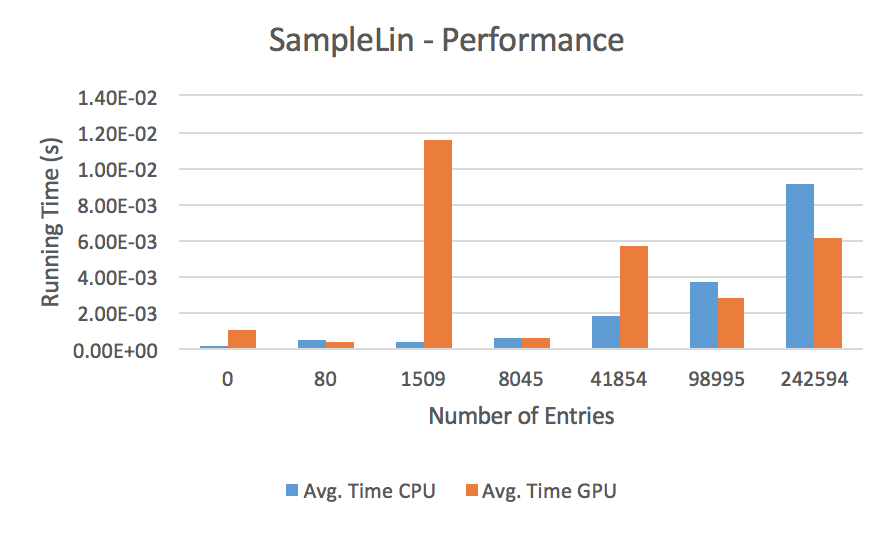
\includegraphics[width=0.7\textwidth]{samplelin_bar.png}
    	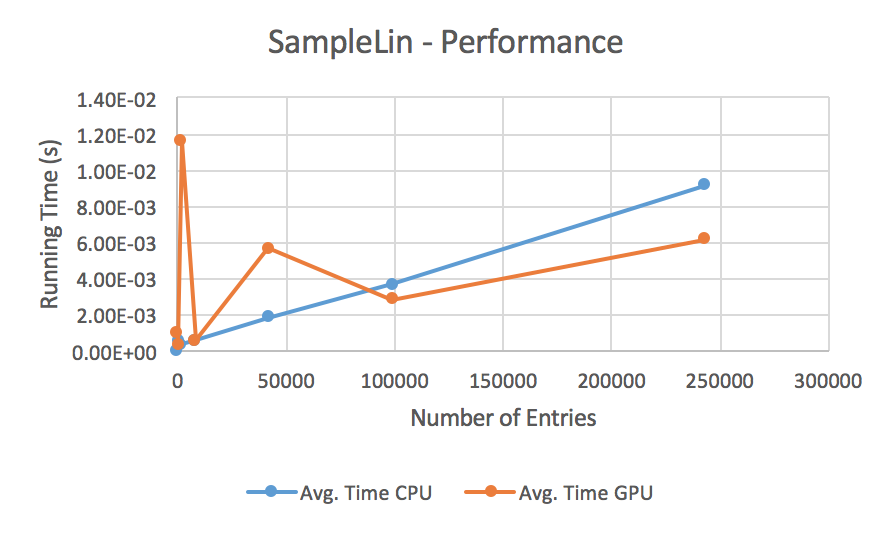
\includegraphics[width=0.7\textwidth]{samplelin_line.png}
    	\end{figure}
	The extraneous point for 1509 entries where the GPU function is significantly slower can be attributed to the need to copy the data from the GPU memory back to CPU memory in this case.

	\subsubsection{Expected vs. Actual output}
		We expected the results on the GPU to be the same as on the CPU. We were also expecting to see SampleLin perform better on the GPU 			as the number of entries in the vector grew\\
	 	The results on the GPU and CPU were both the same, as expected. SampleLin seems to appear to perform better after 100,000 entries.

\subsection{void Times(G4double factor)} % Test Cases done
	
	Multiplies every element in the vector by \texttt{factor}.
	
	\subsubsection{Test Inputs}
		\begin{table}[H]
		\centering
		\caption{Unit Tests - \texttt{Times}}\label{Times_unit}
		\begin{tabular}{lll}
		\toprule
		\multirow{2}{*}{\bf Test \#}  & \multicolumn{1}{c}{\bf Inputs}\\
		& \bf \texttt{factor}\\\midrule
		\refstepcounter{TestCounter}\arabic{TestCounter}\label{Times_0} & r1\\
		\refstepcounter{TestCounter}\arabic{TestCounter}\label{Times_1} & r2\\
		\refstepcounter{TestCounter}\arabic{TestCounter}\label{Times_2} & r3\\
		\refstepcounter{TestCounter}\arabic{TestCounter}\label{Times_3} & r4\\
		\refstepcounter{TestCounter}\arabic{TestCounter}\label{Times_4} & r5\\
		\bottomrule
		\end{tabular}
		\end{table}
	
	\subsubsection{Test Results}
		\begin{table}[H]
		\centering
		\caption{Test Results -- Times}\label{Times_acc}
		\begin{tabular}{clllllll}
		\toprule
		\multirow{2}{*}{\bf Test \#} & \multicolumn{7}{c}{\bf Test Result}\\
		& vec0 & vec1 & vec2 & vec3 & vec4 & vec5 & vec6\\\midrule
		\ref{Times_0} & Pass & Pass & Pass & Pass & Pass & Pass & Pass\\
		\ref{Times_1} & Pass & Pass & Pass & Pass & Pass & Pass & Pass\\
		\ref{Times_2} & Pass & Pass & Pass & Pass & Pass & Pass & Pass\\
		\ref{Times_3} & Pass & Pass & Pass & Pass & Pass & Pass & Pass\\
		\ref{Times_4} & Pass & Pass & Pass & Pass & Pass & Pass & Pass\\
		\bottomrule
		\end{tabular}
		\end{table}

	\subsubsection{Performance}
    	\begin{figure}[H]
    	\centering
    	\caption{Performance results for \texttt{Times} function}\label{figPerformanceTimes}
    	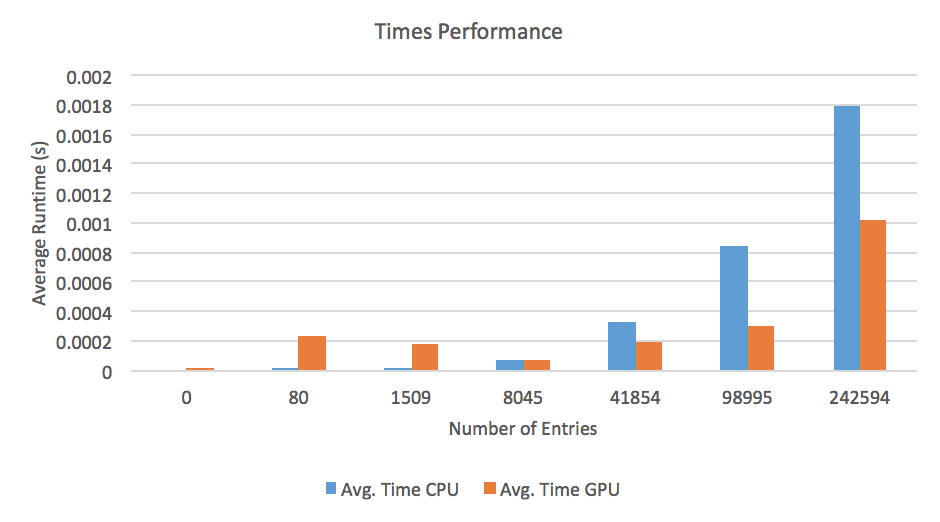
\includegraphics[width=0.7\textwidth]{times_bar.png}
    	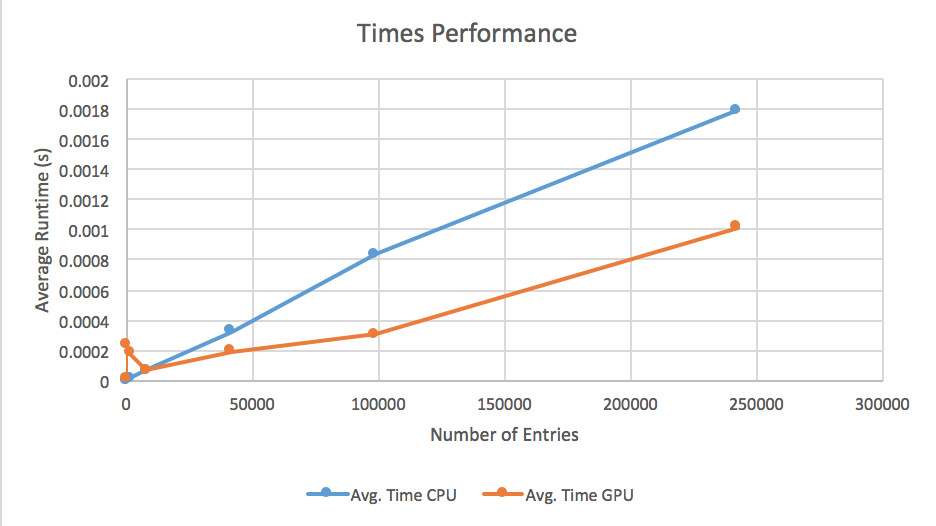
\includegraphics[width=0.7\textwidth]{times_line.png}
    	\end{figure}
	\subsubsection{Expected vs. Actual output}
		 We expected the results on the GPU to be the same as on the CPU. We expected the Times function to run much faster on the GPU 				compared to the CPU\\
	 	The results on the GPU and CPU were both the same, as expected. After roughly 10000 entries the Times function runs faster on the GPU 			compared to the CPU just as expected.

\subsection{void ThinOut(G4double precision)} % Test Cases done 
	
	Removes any element from the vector whose neighbour is closer than \texttt{precision}.
	
	\subsubsection{Test Inputs}
		\begin{table}[H]
		\centering
		\caption{Unit Tests - \texttt{ThinOut}}\label{ThinOut_unit}
		\begin{tabular}{lll}
		\toprule
		\multirow{2}{*}{\bf Test \#}  & \multicolumn{1}{c}{\bf Inputs}\\
		& \bf \texttt{factor}\\\midrule
		\refstepcounter{TestCounter}\arabic{TestCounter}\label{ThinOut_0} & r1\\
		\refstepcounter{TestCounter}\arabic{TestCounter}\label{ThinOut_1} & r2\\
		\refstepcounter{TestCounter}\arabic{TestCounter}\label{ThinOut_2} & r3\\
		\refstepcounter{TestCounter}\arabic{TestCounter}\label{ThinOut_3} & r4\\
		\refstepcounter{TestCounter}\arabic{TestCounter}\label{ThinOut_4} & r5\\
		\bottomrule
		\end{tabular}
		\end{table}
	
	\subsubsection{Test Results}
		\begin{table}[H]
		\centering
		\caption{Test Results -- ThinOut}\label{ThinOut_acc}
		\begin{tabular}{clllllll}
		\toprule
		\multirow{2}{*}{\bf Test \#} & \multicolumn{7}{c}{\bf Test Result}\\
		& vec0 & vec1 & vec2 & vec3 & vec4 & vec5 & vec6\\\midrule
		\ref{ThinOut_0} & Pass & Pass & Pass & Pass & Pass & Pass & Pass\\
		\ref{ThinOut_1} & Pass & Pass & Pass & Pass & Pass & Pass & Pass\\
		\ref{ThinOut_2} & Pass & Pass & Pass & Pass & Pass & Pass & Pass\\
		\ref{ThinOut_3} & Pass & Pass & Pass & Pass & Pass & Pass & Pass\\
		\ref{ThinOut_4} & Pass & Pass & Pass & Pass & Pass & Pass & Pass\\
		\bottomrule
		\end{tabular}
		\end{table}

	\subsubsection{Performance}
		This method is not computationally heavy, so performance data was not included.

	\subsubsection{Expected vs. Actual output}
		 We expected the results on the GPU to be the same as on the CPU.\\
	 	The results on the GPU and CPU were both the same, as expected.



\subsection{G4double GetXsec(G4double e)}
	
	Returns the first xSec from the current vector whose energy is greater than \texttt{e}. 
	
	\subsubsection{Test Inputs}
	Commas denote multiple sub-test inputs. If one of the sub-tests fail then the whole test fails.
		\begin{table}[H]
		\centering
		\caption{Unit Tests - \texttt{GetXsec}}\label{GetXsec_e_unit}
		\begin{tabular}{llll}
		\toprule
		\multirow{2}{*}{\bf Test \#}  & \multicolumn{1}{c}{\bf Inputs}\\
		& \bf \texttt{e}  \\\midrule
		\refstepcounter{TestCounter}\arabic{TestCounter}\label{GetXsec_e_0} & r1, r2, r3, r4, r5 \\
		\refstepcounter{TestCounter}\arabic{TestCounter}\label{GetXsec_e_1} & r1, r2, r3, r4, r5 \\
		\refstepcounter{TestCounter}\arabic{TestCounter}\label{GetXsec_e_2} & r1, r2, r3, r4, r5 \\
		\refstepcounter{TestCounter}\arabic{TestCounter}\label{GetXsec_e_3} & r1, r2, r3, r4, r5 \\
		\refstepcounter{TestCounter}\arabic{TestCounter}\label{GetXsec_e_4} & r1, r2, r3, r4, r5 \\
		\bottomrule
		\end{tabular}
		\end{table}
	
	\subsubsection{Test Results}
		\begin{table}[H]
		\centering
		\caption{Test Results -- GetXsec}\label{GetXsec_e_acc}
		\begin{tabular}{clllllll}
		\toprule
		\multirow{2}{*}{\bf Test \#} & \multicolumn{7}{c}{\bf Test Result}\\
		& vec0 & vec1 & vec2 & vec3 & vec4 & vec5 & vec6\\\midrule
		\ref{GetXsec_e_0} & Pass & Pass & Pass & Pass & Pass & Pass & Pass\\
		\ref{GetXsec_e_1} & Pass & Pass & Pass & Pass & Pass & Pass & Pass\\
		\ref{GetXsec_e_2} & Pass & Pass & Pass & Pass & Pass & Pass & Pass\\
		\ref{GetXsec_e_3} & Pass & Pass & Pass & Pass & Pass & Pass & Pass\\
		\ref{GetXsec_e_4} & Pass & Pass & Pass & Pass & Pass & Pass & Pass\\
		\bottomrule
		\end{tabular}
		\end{table}
	\subsubsection{Performance}
    	\begin{figure}[H]
    	\centering
    	\caption{Performance results for \texttt{GetXSec(e)} function}\label{figPerformanceGetXSec_e}
    	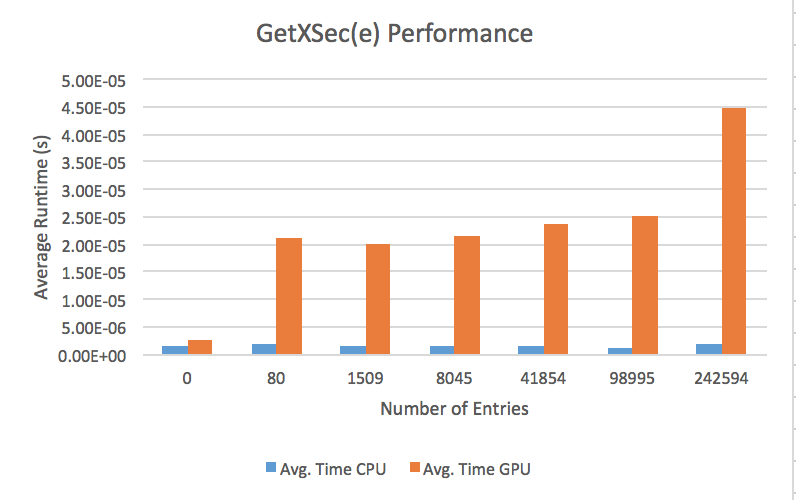
\includegraphics[width=0.7\textwidth]{getxsec_e_bar.png}
    	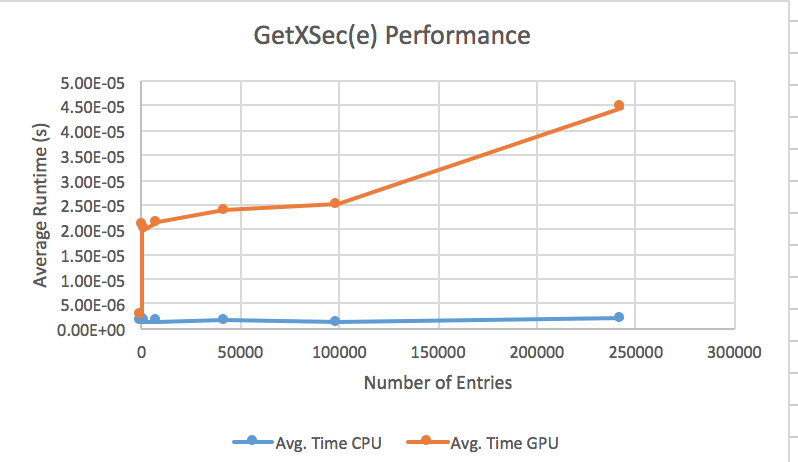
\includegraphics[width=0.7\textwidth]{getxsec_e_line.png}
    	\end{figure}
	The GPU function is significantly slower. This is due to the lack of a hashing function as on the CPU which dramatically speeds up the time to find the first element in the data with energy at least \emph{e}. It can be noted in figure \ref{figPerformanceGetXSec_e_min} that when a minimum value is pre-declared the performance gap is much smaller.

	\subsubsection{Expected vs. Actual output}
		 We expected the results on the GPU to be the same as on the CPU. We expected the function to run faster on the GPU compared to the 			CPU\\
	 	The results on the GPU and CPU were both the same, as expected. Unfortunately, the function performed much worse on the GPU 				compared to the CPU.
	
\subsection{G4double GetXsec(G4double e, G4int min)}
	Returns the first xSec from the current vector whose energy is greater than \texttt{e}. 
	
	\subsubsection{Test Inputs}
	Commas denote multiple sub-test inputs. If one of the sub-tests fail then the whole test fails.
		\begin{table}[H]
		\centering
		\caption{Unit Tests - \texttt{GetXsec}}\label{GetXsec_e_min_unit}
		\begin{tabular}{llll}
		\toprule
		\multirow{2}{*}{\bf Test \#}  & \multicolumn{2}{c}{\bf Inputs}\\
		& \bf \texttt{e} & \bf \texttt{min} \\\midrule
		\refstepcounter{TestCounter}\arabic{TestCounter}\label{GetXsec_e_min_0} & r1, r2, r3, r4, r5 & -1\\
		\refstepcounter{TestCounter}\arabic{TestCounter}\label{GetXsec_e_min_1} & r1, r2, r3, r4, r5 & 0\\
		\refstepcounter{TestCounter}\arabic{TestCounter}\label{GetXsec_e_min_2} & r1, r2, r3, r4, r5 & n/2\\
		\refstepcounter{TestCounter}\arabic{TestCounter}\label{GetXsec_e_min_3} & r1, r2, r3, r4, r5 & n-1\\
		\refstepcounter{TestCounter}\arabic{TestCounter}\label{GetXsec_e_min_4} & r1, r2, r3, r4, r5 & n\\
		\bottomrule
		\end{tabular}
		\end{table}
	
	\subsubsection{Test Results}
		\begin{table}[H]
		\centering
		\caption{Test Results -- GetXsec}\label{GetXsec_e_min_acc}
		\begin{tabular}{clllllll}
		\toprule
		\multirow{2}{*}{\bf Test \#} & \multicolumn{7}{c}{\bf Test Result}\\
		& vec0 & vec1 & vec2 & vec3 & vec4 & vec5 & vec6\\\midrule
		\ref{GetXsec_e_min_0} & Pass & Pass & Pass & Pass & Pass & Pass & Pass\\
		\ref{GetXsec_e_min_1} & Pass & Pass & Pass & Pass & Pass & Pass & Pass\\
		\ref{GetXsec_e_min_2} & Pass & Pass & Pass & Pass & Pass & Pass & Pass\\
		\ref{GetXsec_e_min_3} & Pass & Pass & Pass & Pass & Pass & Pass & Pass\\
		\ref{GetXsec_e_min_4} & Pass & Pass & Pass & Pass & Pass & Pass & Pass\\
		\bottomrule
		\end{tabular}
		\end{table}

	\subsubsection{Performance}
		\begin{figure}[H]
    	\centering
    	\caption{Performance results for \texttt{GetXSec(e,min)} function}\label{figPerformanceGetXSec_e_min}
    	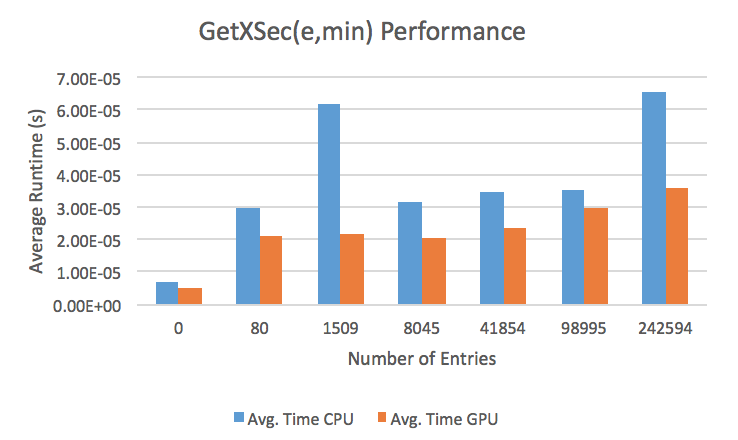
\includegraphics[width=0.7\textwidth]{getxsec_e_min_bar.png}
    	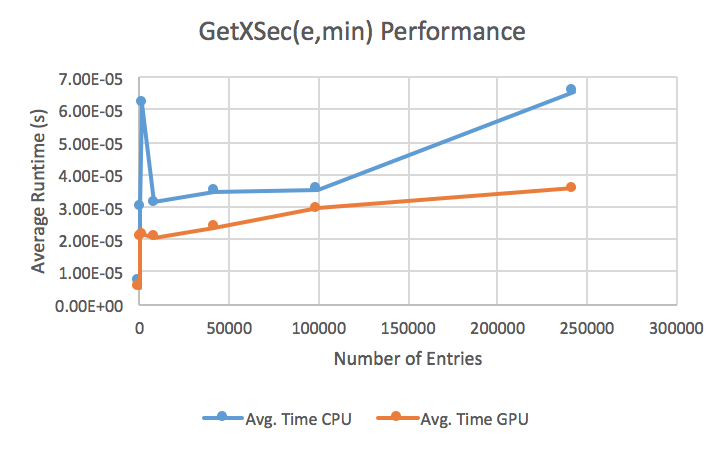
\includegraphics[width=0.7\textwidth]{getxsec_e_min_line.png}
    	\end{figure}

	\subsubsection{Expected vs. Actual output}
		 We expected the results on the GPU to be the same as on the CPU. We expected this function to perform better on the GPU\\
	 	The results on the GPU and CPU were both the same, as expected. This function performed better on the GPU as expected.

\subsection{G4double Get15percentBorder()}
	
	 Returns the integral from each data point to the last data point and returns the first one within 
15\% of the last data point.
	
	\subsubsection{Test Inputs}
		\begin{table}[H]
		\centering
		\caption{Unit Tests - \texttt{Get15percentBorder}}\label{Get15percentBorder_unit}
		\begin{tabular}{lll}
		\toprule
		\multirow{2}{*}{\bf Test \#}  & \multicolumn{1}{c}{\bf Inputs}\\
		& \bf \texttt{N/A}\\\midrule
		\refstepcounter{TestCounter}\arabic{TestCounter}\label{Get15percentBorder_0} & N/A \\
		\bottomrule
		\end{tabular}
		\end{table}
	
	\subsubsection{Test Results}
		\begin{table}[H]
		\centering
		\caption{Test Results -- Get15percentBorder}\label{Get15percentBorder_acc}
		\begin{tabular}{clllllll}
		\toprule
		\multirow{2}{*}{\bf Test \#} & \multicolumn{7}{c}{\bf Test Result}\\
		& vec0 & vec1 & vec2 & vec3 & vec4 & vec5 & vec6\\\midrule
		\ref{Get15percentBorder_0} & Pass & Pass & Pass & Pass & Pass & Pass & Pass\\
		\bottomrule
		\end{tabular}
		\end{table}

	\subsubsection{Performance}
		\begin{figure}[H]
    	\centering
    	\caption{Performance results for \texttt{Get15PercentBorder}}\label{figPerformanceGet15Percent}
    	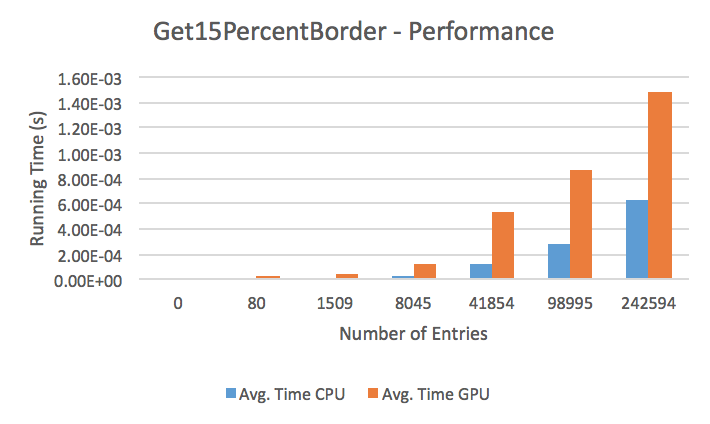
\includegraphics[width=0.7\textwidth]{get15_bar.png}
    	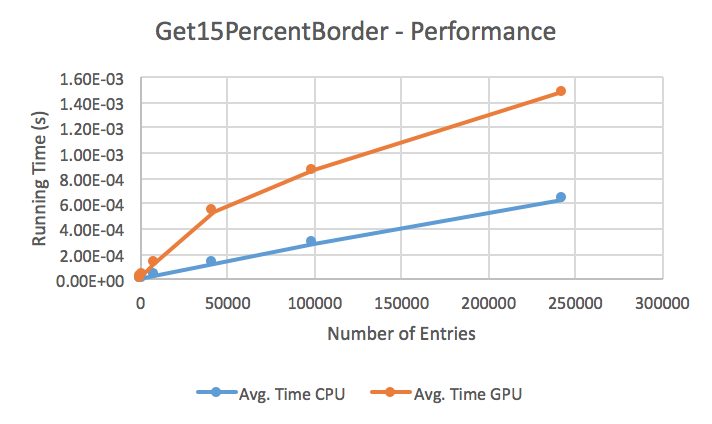
\includegraphics[width=0.7\textwidth]{get15_line.png}
    	\end{figure}

	\subsubsection{Expected vs. Actual output}
		We expected the results on the GPU to be the same as on the CPU. We expected this function to take the same amount of time on the 			GPU as it would take on the CPU.\\
	 	The results on the GPU and CPU were both the same, as expected. The GPU version of this function actually took longer when compared to 		its CPU version counter part.
		
\subsection{G4double Get50percentBorder()}% Test Cases Done
	
	 Returns the integral from each data point to the last data point and returns the first one within 
50\% of the last data point.
	
	\subsubsection{Test Inputs}
		\begin{table}[H]
		\centering
		\caption{Unit Tests - \texttt{Get50percentBorder}}\label{Get50percentBorder_unit}
		\begin{tabular}{lll}
		\toprule
		\multirow{2}{*}{\bf Test \#}  & \multicolumn{1}{c}{\bf Inputs}\\
		& \bf \texttt{N/A}\\\midrule
		\refstepcounter{TestCounter}\arabic{TestCounter}\label{Get50percentBorder_0} & N/A \\
		\bottomrule
		\end{tabular}
		\end{table}
	
	\subsubsection{Test Results}
		\begin{table}[H]
		\centering
		\caption{Test Results -- Get50percentBorder}\label{Get50percentBorder_acc}
		\begin{tabular}{clllllll}
		\toprule
		\multirow{2}{*}{\bf Test \#} & \multicolumn{7}{c}{\bf Test Result}\\
		& vec0 & vec1 & vec2 & vec3 & vec4 & vec5 & vec6\\\midrule
		\ref{Get50percentBorder_0} & Pass & Pass & Pass & Pass & Pass & Pass & Pass\\
		\bottomrule
		\end{tabular}
		\end{table}
		
\ds{As an overall note: Please give each test case its own explicit explanation. 
Seeing tables that say ``Test\#XX -- -- -- --" is not very intuitive or helpful. 
Instead try something like ``Test\#XX (as a heading) then explain that 
parameter1=-1, parameter2=xyz ..." 
and explain the expected vs. actual output.}
\mmp{Added expected vs actual subsection for every function}

	\subsubsection{Performance}
		\begin{figure}[H]
    	\centering
    	\caption{Performance results for \texttt{Get50PercentBorder} function}\label{figPerformanceGet50Percent}
    	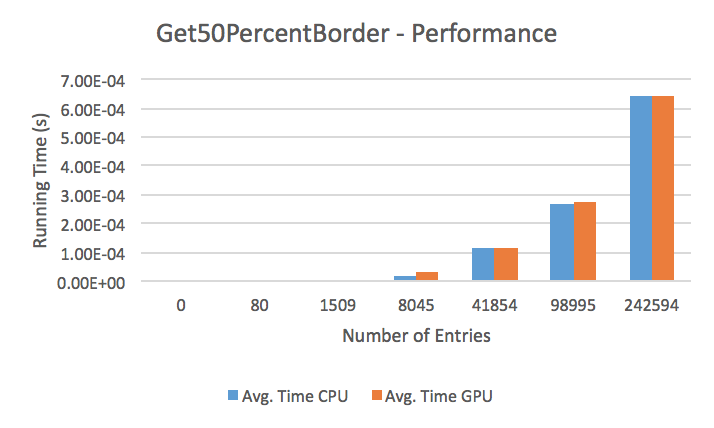
\includegraphics[width=0.7\textwidth]{get50_bar.png}
    	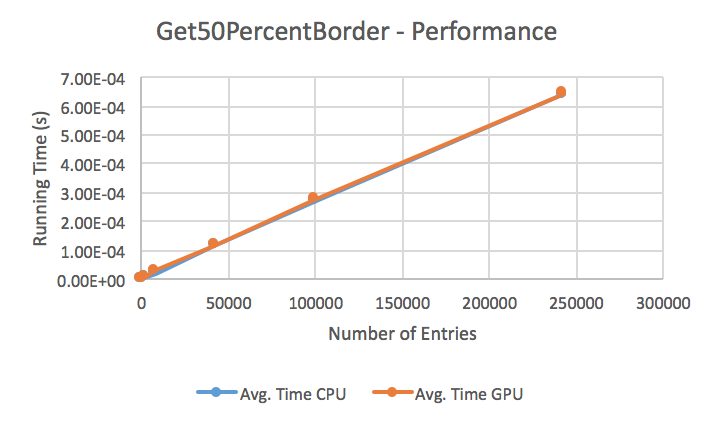
\includegraphics[width=0.7\textwidth]{get50_line.png}
    	\end{figure}

	\subsubsection{Expected vs. Actual output}
		 We expected the results on the GPU to be the same as on the CPU. We expected the performance to be the same on both GPU and CPU\\
	 	The results on the GPU and CPU were both the same, as expected. The performance was the same, as expected on both CPU and GPU.

		
		
% =============================== Section =============================== %
\section{System Tests} \label{System Tests}
\subsection{Summary of System Tests}
System tests are performed by running the sample code packaged with the GEANT4 installation. The Hadr04 example will be run with different materials (i.e water, uranium) and varying number of events. The values and conditions that are changed per test are detailed in table \ref{Table_SystemTests}.\\

For each system test, a summary of the results is recorded. This consists of a section detailing the accuracy of the results, and a section covering performance.. The accuracy of the results will be based on the difference between the values generated on the GPU and the values generated on the CPU. The performance metric that is used is the time required to run each system test.


\begin{center}
\begin{table}[H]
\caption{System Tests}\label{Table_SystemTests}
\begin{tabular}{c>{\raggedright\arraybackslash}p{2.8cm} >{\raggedright\arraybackslash}p{2.8cm}>{\raggedright\arraybackslash}p{3cm}>{\raggedright\arraybackslash}p{3.5cm}}

\toprule
\bf Test \# & \bf Name & \bf Inputs & \bf Same as non-GPU GEANT4 & \bf Description\\\midrule
\refstepcounter{TestCounter}\arabic{TestCounter}\label{sys1}
& System Test - Water, 2000 events
& Events = 2000
Material = Water
& True 
&  Hadr04 no changes\\\midrule

\refstepcounter{TestCounter}\arabic{TestCounter}\label{sys2}
& System Test - Uranium, 2000 events
& Events = 2000
Material = Uranium
& True 
& Hadr04 -- basic example\\\midrule

\refstepcounter{TestCounter}\arabic{TestCounter}\label{sys3}
& System Test - Water, 600 events
& Events = 600
Material = Water
& True 
& Hadr04 -- Shorter test \\\midrule

\refstepcounter{TestCounter}\arabic{TestCounter}\label{sys4}
& System Test - Uranium, 600 events
& Events = 600
Material = Uranium
& True 
& Hadr04 -- Shorter test \\\midrule

\refstepcounter{TestCounter}\arabic{TestCounter}\label{sys5}
& System Test - Uranium, 20000 events
& Events = 20000
Material = Uranium
& True 
& Hadr04 -- Long simulation stress Test\\

\bottomrule

\end{tabular}
\end{table}
\end{center}

\ds{A boolean summary of whether the outputs were accurate (ie. ``Output is the same as CPU GEANT4" -- true/false could be useful instead of your current setup).}
\mmp{Changed to boolean summary}

\subsection{System Test - Water, 2000 events}
This test runs the Hadr04 example on both the GPU and the CPU. The code for the Hadr04 example is bundled with the GEANT4 installation.
	\subsubsection{Accuracy}
	Test output for water, 2000 events:
		\begin{table}[H]
		\centering
		\caption{Accuracy - Water, 2000 events}\label{sys1Acc}
		\begin{tabular}{llll}
		\toprule
		\bf Data & \bf CPU Values & \bf GPU Values & \bf Absolute Difference\\\midrule
		\bf Process Calls&&&\\
		hadElastic&423181&423181&0\\
		nCapture&1998&1998&0\\
		neutronInelastic&2&2&0\\ 

		\midrule
		\bf Parcours of incident neutron&&&\\
		collisions&212.59&212.59&0\\
		track length&93.387 cm&93.387 cm&0\\
		time of flight&202.14 mus&202.14 mus&0\\
	
		\midrule
		\bf Generated particles&&&\\

		\bf{C14}&&&\\
		\# of particles&2&2&0\\
		Emean&404.13 keV&404.13 keV&0\\

		\bf{O16}&&&\\
		\# of particles&5948&5948&0\\
		Emean&39.577 keV&39.577 keV&0\\
		
		\bf{O17}&&&\\
		\# of particles&4&4&0\\
		Emean&1.4823 keV&1.4823 keV&0\\
		
		\bf{O18}&&&\\
		\# of particles&3&3&0\\
		Emean&52.362 keV&52.362 keV&0\\
		
		\bf{Alpha}&&&\\
		\# of particles&2&2&0\\
		Emean&1.4146 MeV&1.4146 MeV&0\\
		
		\bf{Deuteron}&&&\\
		\# of particles&1996&1996&0\\
		Emean&1.3185 keV&1.3185 keV&0\\
		
		\bf{Gamma}&&&\\
		\# of particles&2000&2000&0\\
		Emean&2.2239 MeV&2.2239 MeV&0\\
		
		\bf{Proton}&&&\\
		\# of particles&45355&45355&0\\
		Emean&83.046 keV&83.046 keV&0\\\bottomrule
		
		\end{tabular}
		\end{table}	

	\subsubsection{Performance}
		\begin{table}[H]
		\centering
		\caption{Performance - Water, 2000 events}\label{_acc}
		\begin{tabular}{lll}
		\toprule
		\bf CPU Time&\bf  GPU Time&\bf Speedup of GPU\\\midrule
		54.55s&72.08s&-1.32$\times$\\\bottomrule
		\end{tabular}
		\end{table}

\subsection{System Test - Uranium, 2000 events}
This test runs the Hadr04 example on both the GPU and the CPU including Uranium as an element in the simulation. The number of events for this test has been set to 2000.
	\subsubsection{Accuracy}
		\begin{table}[H]
		\centering
		\caption{Accuracy - Uranium, 2000 events}\label{sys2Acc}
		\begin{tabular}{llll}
		\toprule
		\bf Data & \bf  CPU Values &  \bf GPU Values &  \bf Absolute Difference\\\midrule
		\bf Process Calls&&&\\
		hadElastic&1931&1931&0\\
		nCapture&29&29&0\\
		nFission&281&281&0\\		
		neutronInelastic&1690&1690&0\\ 

		\midrule	
		\bf Parcours of incident neutron&&&\\
		collisions&1.9655&1.966&0\\
		track length&5.6484 cm&5.6517 cm&0\\
		time of flight&2.896 ns&2.8983 ns&0\\
		
		\midrule
		\bf Generated particles&&&\\
		\bf{U235}&&&\\
		\# of particles&29&29&0\\
		Emean&6.5841 keV&6.5841 keV&0\\
		
		\bf{U238}&&&\\
		\# of particles&3592&3592&0\\
		Emean&8.8059 keV&8.8059 keV&0\\
		
		\bf{U239}&&&\\
		\# of particles&29&29&0\\
		Emean&8.3978 keV&8.3978 keV&0\\
		
		\bf{Gamma}&&&\\
		\# of particles&4319&4319&0\\
		Emean&496.96 keV&496.96 keV&0\\
		
		\bf{Neutron}&&&\\
		\# of particles&2449&2449&0\\
		Emean&1.2746 MeV&1.2746 MeV&0\\\bottomrule
		
		\end{tabular}
		\end{table}

		\subsubsection{Performance}
		\begin{table}[H]
		\centering
		\caption{Performance - Uranium, 2000 events}\label{sys2Perf}
		\begin{tabular}{lll}
		\toprule
		 \bf CPU Time&  \bf GPU Time& \bf Speedup of GPU\\\midrule
		0.63s&10.57s&-16.78$\times$\\\bottomrule
		\end{tabular}
		\end{table}

\subsection{System Test - Water, 600 events}
This test runs the Hadr04 example on both the GPU and the CPU. The number of runs for this test has been set to 600.

	\subsubsection{Accuracy}
		\begin{table}[H]
		\centering
		\caption{Accuracy - Water, 600 events}\label{sys3Acc}
		\begin{tabular}{llll}
		\toprule
		\bf Data &  \bf CPU Values & \bf  GPU Values & \bf Absolute Difference\\\midrule
		\bf Process Calls&&&\\
		hadElastic&131588&131588&0\\
		nCapture&600&600&0\\
	
		\midrule
		\bf Parcours of incident neutron&&&\\
		collisions&220.31&220.31&0\\
		track length&96.495 cm&96.495 cm&0\\
		time of flight&210.57 mus&210.57 mus&0\\

		\midrule
		\bf Generated particles&&&\\
		\bf{O16}&&&\\
		\# of particles&1819&1819&0\\
		Emean&41.788 keV&41.788 keV&0\\
		
		\bf{O17}&&&\\
		\# of particles&3&3&0\\
		Emean&316.87 eV&316.87 eV&0\\
		
		\bf{O18}&&&\\
		\# of particles&1&1&0\\
		Emean&9.3256 eV&9.3256 eV&0\\	
		\bf{Deuteron}&&&\\
		\# of particles&597&597&0\\
		Emean&1.319 keV&1.319 keV&0\\	
		\bf{Gamma}&&&\\
		\# of particles&602&602&0\\
		Emean&2.2229 MeV&2.2229 MeV&0\\	
		\bf{Proton}&&&\\
		\# of particles&13860&13860&0\\
		Emean&81.141 keV&81.141 keV&0\\\bottomrule
		\end{tabular}
		\end{table}

	\subsubsection{Performance}
		\begin{table}[H]
		\centering
		\caption{Performance - Water, 600 events}\label{sys3Perf}
		\begin{tabular}{lll}
		\toprule
		 \bf CPU Time&  \bf GPU Time& \bf Speedup of GPU\\\midrule
		17.07s&22.11s&-1.29$\times$\\\bottomrule
		\end{tabular}
		\end{table}
		
\subsection{System Test - Uranium, 600 events}
This test runs the Hadr04 example on both the GPU and the CPU with a modified source files to include Uranium as an element is the simulation. The number of events is set to 600, a lower number of events than the other tests, to see how fewer events will impact accuracy and performance.
	\subsubsection{Accuracy}
		\begin{table}[H]
		\centering
		\caption{Accuracy - Uranium, 600 events}\label{sys4Acc}
		\begin{tabular}{llll}
		\toprule
		\bf Data &  \bf CPU Values &  \bf GPU Values &  \bf Absolute Difference\\\midrule
		\bf Process Calls&&&\\
		hadElastic&562&562&0\\
		nCapture&8&8&0\\
		nFission&89&89&0\\
		neutronInelastic&508&508&0\\ 

		\midrule
		\bf Parcours of incident neutron&&&\\
		collisions&1.9367&1.9367&0\\
		track length&5.6204 cm&5.6204 cm&0\\
		time of flight&2.8817 ns&2.8817 ns&0\\

		\midrule
		\bf Generated particles&&&\\
		
		\bf{U235}&&&\\
		\# of particles&6&6&0\\
		Emean&6.131 keV&6.131 keV&0\\
		
		\bf{U238}&&&\\
		\# of particles&1064&1064&0\\
		Emean&8.9857 keV&8.9857 keV&0\\
		
		\bf{U239}&&&\\
		\# of particles&8&8&0\\
		Emean&8.3308 keV&8.3308 keV&0\\
		
		\bf{Gamma}&&&\\
		\# of particles&1261&1261&0\\
		Emean&486.58 keV&47486.58 keV&0\\
		
		\bf{Neutron}&&&\\
		\# of particles&743&743&0\\
		Emean&1.3038 MeV&1.3038 MeV&0\\\bottomrule
		\end{tabular}
		\end{table}

	\subsubsection{Performance}
		\begin{table}[H]
		\centering
		\caption{Performance - Uranium, 600 events}\label{sys4Perf}
		\begin{tabular}{lll}
		\toprule
		 \bf CPU Time&  \bf GPU Time& \bf Speedup of GPU\\\midrule
		0.22s&3.01s&-13.68$\times$\\\bottomrule
		\end{tabular}
		\end{table}

\subsection{System Test - Uranium, 20000 events}
This test runs the Hadr04 example on both the GPU and the CPU including Uranium as an element in the simulation. The number of events is set to 20000. The idea is to see if speed and accuracy gaps will widen or shrink as the number of events increases.

	\subsubsection{Accuracy}
		\begin{table}[H]
		\centering
		\caption{Accuracy - Uranium, 20000 events}\label{sys5Acc}
		\begin{tabular}{llll}
		\toprule
		\bf Data &  \bf CPU Values &  \bf GPU Values &  \bf Absolute Difference\\\midrule
		\bf Process Calls&&&\\
		hadElastic&19526&19526&0\\
		nCapture&245&245&0\\
		nFission&2933&2933&0\\
		neutronInelastic&16822&16822&0\\ 
		
		\midrule
		\bf Parcours of incident neutron&&&\\
		collisions&1.9763&1.9763&0\\
		track length&5.6512 cm&5.6512 cm&0\\
		time of flight&2.898 ns&2.898 ns&0\\

		\midrule
		\bf Generated particles&&&\\
		\bf{U234}&&&\\
		\# of particles&6&6&0\\
		Emean&3.1299 keV&3.1299 keV&0\\
		
		\bf{U235}&&&\\
		\# of particles&223&223&0\\
		Emean&8.4136 keV&8.4136 keV&0\\
		
		\bf{U236}&&&\\
		\# of particles&2&2&0\\
		Emean&9.5669 keV&9.5669 keV&0\\
		
		\bf{U238}&&&\\
		\# of particles&36119&36119&0\\
		Emean&8.8767 keV&8.8767 keV&0\\
		
		\bf{U239}&&&\\
		\# of particles&243&243&0\\
		Emean&8.428 keV&8.428 keV&0\\
		\bf{Gamma}&&&\\
		\# of particles&43826&43826&0\\
		Emean&479.54 keV&479.54 keV&0\\
		\bf{Proton}&&&\\
		\# of particles&24374&24374&0\\
		Emean&1.2749 MeV&1.2749 MeV&0\\\bottomrule
		\end{tabular}
		\end{table}

	\subsubsection{Performance}
		\begin{table}[H]
		\centering
		\caption{Performance - Uranium, 20000 events}\label{sys5Perf}
		\begin{tabular}{lll}
		\toprule
		\bf CPU Time& \bf GPU Time& \bf Speedup on GPU\\\midrule
		6.4s&106.41s&-16.64$\times$\\\bottomrule
		\end{tabular}
		\end{table}		

% =============================== Section =============================== %
\section{Traceability}\label{Traceability}
The following section is used to highlight the relations of implemented test cases to requirements and modules. In doing so, we hope to draw clear reasoning upon the inclusion of such tests. 

\subsection{Requirements}
Below is a traceability table outlining test cases and the requirements they are related to:\\

\begin{center}
\begin{longtable}{>{\raggedright\arraybackslash}p{0.1\textwidth}>{\raggedright\arraybackslash}p{0.3\textwidth}>{\raggedright\arraybackslash}p{0.5\textwidth}}
\caption{Tests and Requirements Relationship}\label{Table_TestsAndRequirements}
\\\toprule
\bf Test \#  & \bf Description & \bf Requirement\\\midrule
\ref{Init_0}, \ref{SampleLin_0}, \ref{Times_0}, \ref{GetXsec_e_0} - \ref{GetXsec_e_4}, \ref{GetXsec_e_min_0} - \ref{GetXsec_e_min_4}, \ref{Get15percentBorder_0}, \ref{Get50percentBorder_0} & Unit tests, with performance measured & Req. \# 4 (Speed and Latency)\\
\ref{sys1} - \ref{sys5} & System tests, with performance measured & Req. \# 4 (Speed and Latency)\\
\ref{Init_0} - \ref{Get50percentBorder_0} & Unit tests, with accuracy measured & Req \# 5, 6, 7 (Precision, Reliability, Robustness)\\
\ref{sys1} - \ref{sys5} & System tests, with accuracy measured & Req \# 5, 6, 7 (Precision, Reliability, Robustness)\\
\bottomrule
\end{longtable}
\end{center}
\subsection{Modules}
Similarly, the following is a traceability table explicitly relating test cases to modules:\\

\begin{center}
\begin{longtable}{>{\raggedright\arraybackslash}p{0.1\textwidth}>{\raggedright\arraybackslash}p{0.3\textwidth}>{\raggedright\arraybackslash}p{0.5\textwidth}}
\caption{Tests and Modules Relationship}\label{Table_TestsAndModules}
\\\toprule
\bf Test \#  & \bf Description & \bf Module\\\midrule
\ref{Init_0} - \ref{Get50percentBorder_0} & Unit tests & G4ParticleVector\\
\ref{sys1} - \ref{sys5} & System tests & G4ParticleHPDataPoint, G4ParticleVector, CMake Files\\
\bottomrule
\end{longtable}
\end{center}

% =============================== Section =============================== 
% --------------------------- Stuart
\section{Changes after Testing}\label{Changes after Testing}
Developing the unit testing system illuminated a variety of bugs and changes that needed to be made. These were predominantly related to edge cases -- trying to access indices in arrays that are negative or greater than the number of elements in the array was a common theme. Some of these edge cases were not covered by Geant4 itself, so the required change was made to the original Geant4 source code as well as the modified CUDA code.\\

Aside from the handling of edge cases with if guards, there was one more significant change required to get the unit tests to pass. An important control flow statement in \texttt{GetXSec(e,min)} was supposed to branch if the difference between two values was below a certain threshold. Our implementation was missing a call to get the absolute value for this difference, and as such was returning the wrong result in cases where the second value was larger than the first.\\

In terms of performance, some performance testing had been done prior to the development of the unit testing system. That profiling data led us to reimplement nearly every function on the GPU using a hybrid approach wherein the data values are stored in both GPU and CPU memory, are modified mainly on the GPU and then the version in CPU memory is updated only when required. This gave very large performance improvements, with the GPU code going from ~4.5X slower to ~1.2X slower for the Hadr04 example. Further performance tuning is planned for the future based on the results from individual unit tests.


\end{document}
